\documentclass[a4paper]{article}

%% Language and font encodings
\usepackage[spanish]{babel}
\usepackage[utf8x]{inputenc}
\usepackage[T1]{fontenc}
\usepackage{listings}
\spanishdecimal{.}


%% Sets page size and margins
\usepackage[a4paper,top=3cm,bottom=2cm,left=3cm,right=3cm,marginparwidth=1.75cm]{geometry}

%% Useful packages
\usepackage{amsmath}
\usepackage{graphicx}
\usepackage[colorinlistoftodos]{todonotes}
\usepackage[colorlinks=true, allcolors=blue]{hyperref}

\title{Práctica 4: diagramas de Voronoi}
\date{}
\begin{document}

\maketitle

\section{Introducci\'on}
Se tiene una rejilla o malla de medidas $n\times n$ determinadas, y buscaremos definir bien celdas de Voronoi en base a ésta, es decir, dejaremos que dentro de esta malla existan o <<nazcan>> $k$ semillas, las cuales en un inicio parecerán solo puntos sobre nuestro sistema, pero al final cada punto de la rejilla es asignado a una semilla, es decir se forman las celdas. En el sistema tambien existen <<grietas>>, es decir existe una probabilidad de que se desarrolle una grieta entre mis celdas, mientras la grieta se propague por los bordes de las celdas, tiene una mayor probabilidad de seguir creciendo, el objetivo de la práctica en general será examinar el efecto de la variación de semillas en el sistema, así como el tamaño de las zonas con el fin de observar el comportamiento de los largos de las grietas.

\section{Par\'ametros de trabajo}
La experiemtnación se realizó en un HP Z230 Tower Workstation con procesador Intel(R) Xenon(R) CPU E3-1240 v3 y 3.40 GHz de memoria ram 16 GB y un sistema operativo de 64 bits con Windows 7 Home Premium.

Se tiene una rejilla de $n\times n$,  $n \in \{40, 100, 200\} $ y se esparcen $k \in \{12,20,50,70,100\}$ semillas, se toma la misma medida para conciderar a una grieta como tal, que el número de pasos que da, es decir su largo sea suprior o igual a la dimensión $n$, considerandola así lo suficiente mente larga para su observación

\section{Modificaciones del código}
Se incluyeron unicamente dos ciclos \texttt{for} para la automatización de las medias, uno encargado de variar la cantidad de semillas en la malla y el otro encargado de variar la medida de ella. Así mismo se incluyeron dos vectores con el fin de almacenar los valores que toman $k$ y $n$. Así como se agregó la librería \texttt{ggplot} para las gráficas a generar.

\begin{lstlisting}[frame=single]
library('ggplot2')
va <- c(40,100,200)
semillitas<-c(12,20,50,70,100)
for( a in 1:length(va)){
n <- va[a]
for(b in 1:length(semillitas)){
k <- semillitas[b]
\end{lstlisting}

Se crearon también dos \texttt{data.frame}, uno con el fin de guardar los valores de los largos de las grieta en las diferentes combinaciones de parámetros.
\begin{lstlisting}[frame=single]
datos <- data.frame()
dato <- data.frame()
...
dato <- cbind(rep(n,length(largos)),rep(k,length(largos)),largos)
datos <- rbind(datos,dato)
\end{lstlisting}

\section{Resultados y conclusiones}
Los largos de las grietas para las combinaciones de parámetros los podemos ver con mayor claridad en la figura \ref{fig:DistanciasM} podemos observar que hay una ligera variación respecto a la malla de $40 \times 40$, en cambio, la diferencia no es tan notoria con la figura \ref{fig:DistanciasS} donde la cantidad de semillas no parece importar respecto a lo largo de las grietas.
\begin{figure}[h]
\centering
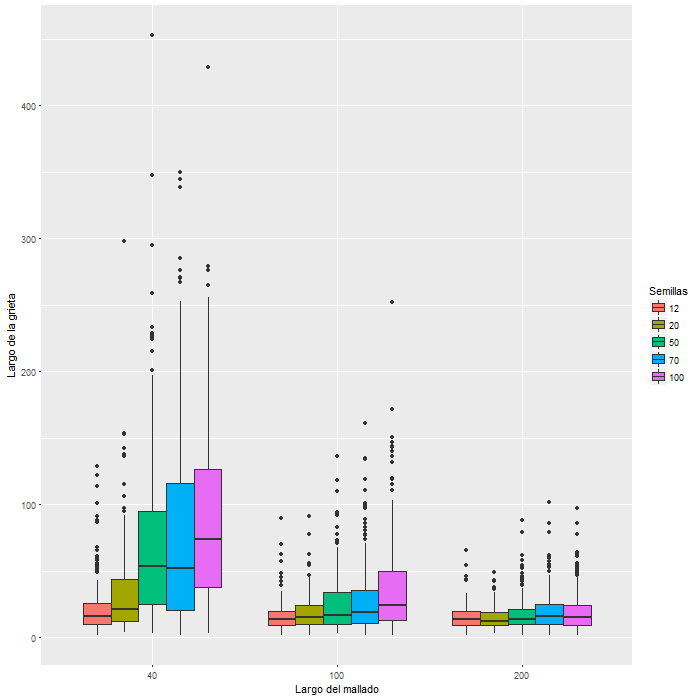
\includegraphics[width=0.7\linewidth]{DistanciasM}
\caption{Largo de las grietas respecto a la dimensión de la malla.}
\label{fig:DistanciasM}
\end{figure}
\begin{figure}[h]
\centering
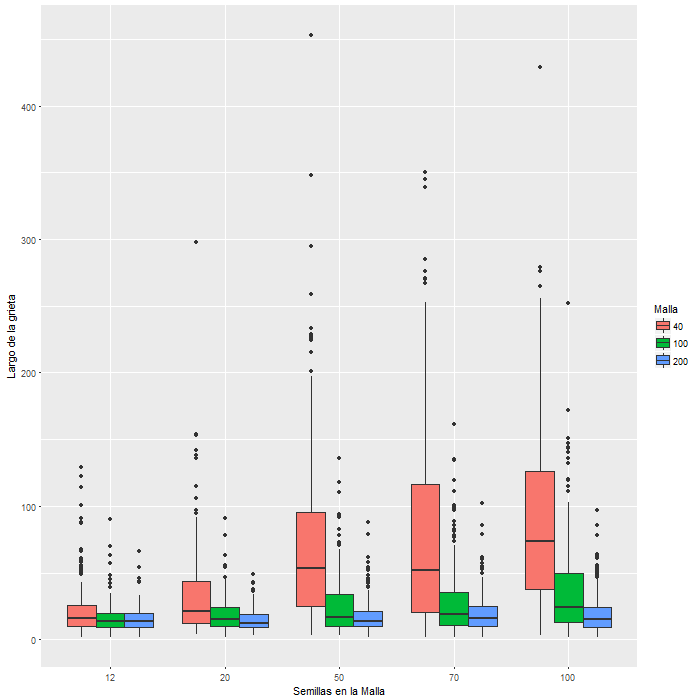
\includegraphics[width=0.7\linewidth]{DistanciasS}
\caption{Largo de las grietas respecto a la cantidad de semillas que se utilizan.}
\label{fig:DistanciasS}
\end{figure}

Se realizaron pruebas de medias en ambos casos con el fin de determinar si efectivamente la dimensión del mallado tenía un efecto significativo, así mismo con la cantidad de semillas, y efectivamente se llega a la conclusión que el mallado afecta, al ser más pequeño la longitud de las grietas es mayos, en cambio no difiere mucho respecto a la cantidad de semillas puesta en él.



\end{document}